\documentclass[12pt,a4paper]{article}

\usepackage[utf8]{inputenc}
\usepackage[brazilian]{babel}
\usepackage{amsmath}
\usepackage{graphicx}
\usepackage{longtable}
\usepackage{siunitx}
\usepackage{booktabs}
\usepackage{geometry}
\usepackage{float}
\usepackage{indentfirst}
\usepackage{newtxtext}
\usepackage{newtxmath}

\usepackage[authoryear]{natbib}

\geometry{margin=2.5cm}

\title{Análise do Movimento Harmônico Amortecido}
\author{Enzo Rocha Leite Diniz Ribas \\ Centro Federal de Educação Tecnológica de Minas Gerais}
\date{\today}

\begin{document}
\begin{titlepage}

\begin{center}


\includegraphics[width=4cm]{media/Logo_CEFET-MG.png}

\Large
Centro Federal de Educação Tecnológica de Minas Gerais

\vspace{1cm}

\Large
Curso de Engenharia Mecânica

\vspace{2cm}

\Huge \textbf{Determinação da velocidade do som no ar através da ressonância acústica em tubos semiabertos}\\[1cm]

\vspace{3cm}

\begin{flushright}
\Large
Mecânica, Oscilações, Fluidos e Termodinâmica, Turma T03 \\
Prof. Dr. Mauro Lucio Lobão Iannini
\end{flushright}

\vspace{3cm}

\large
Enzo Rocha Leite Diniz Ribas (Eng. Mecânica - 20253002819)\\
Gabriel Resende Amorim Oliveira (Eng. Elétrica - 20233014438)\\
Leandro Césari e Silva Barros (Eng. Mecânica - 20253005104)\\

\vfill

\Large
Belo Horizonte

\Large
\the\year/{1}

\end{center}

\end{titlepage}

\section{Introdução}
O roteiro do experimento \citep{Roteiro_Experimento_08} propõe a determinação empírica da velocidade de propagação de uma onda sonora no ar confinada em um tubo semiaberto. A prática tem como objetivo analisar a correlação entre a frequência acústica de excitação e o comprimento da coluna de ar ressonante, além de investigar quantitativamente os efeitos de borda (correção de extremidade) associados à geometria do tubo de ensaio e da caixa de ressonância. O experimento também propõe uma avaliação crítica das limitações físicas e fisiológicas do método tradicional, visando propor um modelo de medição eletroacústica de precisão. propõe a análise do movimento harmônico amortecido com o objetivo de "Analisar a dependência com o tempo da amplitude do movimento harmônico de um sistema massa-mola amortecido'' e "determinar o coeficiente de amortecimento e outras constantes descritivas do movimento oscilatório''.

\section{Fundamentação Teórica}
\subsection{Propagação Ondulatória e Velocidade do Som no Ar}
A relação cinemática fundamental para o movimento ondulatório liga a velocidade de fase $v$, o comprimento de onda $\lambda$ e a frequência de oscilação $f$:
\begin{equation}
    v = \lambda \cdot f
\end{equation}

A velocidade de propagação em um gás ideal é estritamente dependente de suas propriedades termodinâmicas, sendo equacionada de forma rigorosa por:
\begin{equation}
    v = \sqrt{\frac{\gamma \cdot R \cdot T}{M}}
\end{equation}

Onde $\gamma$ é a razão dos calores específicos do ar ($\gamma = 1,4$), $R = 8,31\text{ J/(mol}\cdot\text{K)}$ é a constante universal dos gases, $T$ é a temperatura absoluta em Kelvin e $M \approx 28,96 \times 10^{-3}\text{ kg/mol}$ é a massa molar média do ar. 

\subsection{Termometria Termoelétrica (O Efeito Seebeck)}
Para a determinação da temperatura ambiente ($T$), utilizou-se uma sonda termopar tipo K conectada a um multímetro digital. O funcionamento desse instrumento é baseado no Efeito Seebeck. A imposição de um gradiente térmico entre a junção exposta ao ar e a junção de referência induz uma difusão desigual de elétrons livres, gerando uma força eletromotriz (f.e.m.) térmica na escala de microvolts ($\mu\text{V}$), cuja magnitude é descrita pela integral analítica:
\begin{equation}
    V_{\text{Seebeck}} = \int_{T_{\text{ref}}}^{T_{\text{sonda}}} (S_{\text{A}} - S_{\text{B}})\, dT
\end{equation}

\subsection{Física da Fonte Acústica (O Diapasão Metálico)}
O diapasão atua como o padrão primário de frequência ($440\text{ Hz}$) do experimento. Fisicamente, cada uma de suas hastes se comporta como uma viga engastada sujeita à flexão. A frequência natural de oscilação flexional para este modelo contínuo é extraída da equação de Euler-Bernoulli:
\begin{equation}
    f_{\text{natural}} \propto \frac{h}{L_{\text{haste}}^2} \sqrt{\frac{E}{\rho}}
\end{equation}
Como essas variáveis geométricas e mecânicas são rigidamente fixas na usinagem da peça, a frequência emitida não sofre flutuações.

\subsection{Acústica Musical e o Cálculo de Frequências}
Para a varredura no tubo, o grupo estruturou a coleta baseando-se na escala musical de Temperamento Igual. Adotando a frequência nominal do diapasão ($A_4$) como referência ($f_{\text{ref}} = 440\text{ Hz}$), a frequência $f_n$ de qualquer outra nota adjacente é obtida pela equação fundamental:
\begin{equation}
    f_n = f_{\text{ref}} \cdot 2^{\frac{n}{12}} = 440 \cdot 2^{\frac{n}{12}}
\end{equation}
Onde $n$ é o número de semitons de distância até o Lá de referência. Essa previsibilidade ditou os valores inseridos no gerador de tons, garantindo um espaçamento exponencial e consistente.

\subsection{A Caixa de Ressonância e a Discrepância Dimensional}
Acopla-se ao diapasão uma caixa oca de madeira (aberta em uma extremidade) para amplificar o som. A condição de contorno para o primeiro modo harmônico exige um nó de pressão na abertura e um ventre na parede fechada:
\begin{equation}
    L_{\text{caixa}} = \frac{\lambda}{4} = \frac{v}{4f}
\end{equation}

Contudo, devido à inércia do ar, a massa do fluido na abertura oscila além dos limites físicos da caixa (Correção de Extremidade). Logo, o comprimento da caixa medido com a régua ($L_{\text{interno}}$) será sempre numericamente inferior ao comprimento acústico confinado.

\subsection{Ressonância Variável no Tubo D'água}
No ensaio, o tubo de acrílico imerso em água atua como um ressonador de comprimento variável, com a água funcionando como um nó de deslocamento rígido. Para o modo fundamental ($n=1$), a relação é regida por:
\begin{equation}
    L = \left(\frac{v_{\text{tubo}}}{4}\right) \cdot \frac{1}{f}
\end{equation}

\section{Metodologia}

O experimento foi realizado utilizando os seguintes materiais:
\begin{itemize}
    \item \textit{Smartphone} com o aplicativo \textit{PhyPhox};
    \item Multímetro digital com sonda termopar tipo K;
    \item Diapasão de metal de $440\text{ Hz}$ e caixa de ressonância;
    \item Tubo de acrílico cilíndrico e recipiente com água;
    \item Régua milimetrada metálica ($\pm 0,001\text{ m}$).
\end{itemize}

\begin{figure}[htbp]
  \centering
  
\includegraphics[width=.8\linewidth]{media/photos/sistema}
  \caption{Montagem experimental da bancada.}
  \label{fig:montagem}
\end{figure}

\section{Procedimentos Experimentais}

\subsection{Condições Iniciais e Geométricas}
Posicionou-se o termopar no centro do laboratório, aguardando a estabilização térmica para o registro da temperatura ambiente. Em seguida, com a régua milimetrada, mediu-se o comprimento interno da caixa de ressonância ($L_{\text{interno}}$) para estabelecer a discrepância frente à onda de $440\text{ Hz}$.

\subsection{Coleta de Dados e Restrições Físicas do Tubo}
O tubo de acrílico possuía um comprimento total medido de $35,3\text{ cm}$. Ao iniciar o experimento, o tubo colidia com o fundo plástico do recipiente, inviabilizando a verificação de colunas de ar curtas. Diante desta restrição, utilizou-se o equacionamento da oitava musical (Eq. 5) para calcular e predeterminar frequências que resultassem em comprimentos fisicamente ajustáveis. A varredura foi direcionada de $528\text{ Hz}$ a $294\text{ Hz}$. 

É importante destacar a justificativa física que garante que as leituras referem-se estritamente ao modo fundamental ($n=1$). Sabendo que a ressonância para $440\text{ Hz}$ exige $L_1 \approx 19,6\text{ cm}$, o próximo harmônico ímpar ($n=3$) ocorreria apenas em $L_3 \approx 3 \times 19,6 = 58,8\text{ cm}$. Como $58,8\text{ cm} > 35,3\text{ cm}$, comprova-se matematicamente que a dimensão máxima do tubo atua como um filtro físico, impossibilitando a excitação de harmônicos superiores.


\section{Apresentação e Análise de Resultados}

\subsection{Parâmetros Termodinâmicos Rigorosos}
\begin{itemize}
    \item Temperatura no centro do laboratório: $T = 24,5^\circ\text{C}$
    \item Temperatura absoluta: $T = 297,65\text{ K}$
    \item Velocidade Teórica do som (usando a Equação 2 completa):
\end{itemize}
\begin{equation}
    v_{\text{teorica}} = \sqrt{\frac{1,4 \cdot 8,31 \cdot 297,65}{28,96 \times 10^{-3}}} \approx 345,88\text{ m/s}
\end{equation}

A evaporação da água no interior do cano implica em uma pequena redução local de temperatura, justificando desvios sutis na medição prática da velocidade em relação a esta referência da sala livre.

\subsection{Correção de Borda na Caixa de Ressonância}
\begin{itemize}
    \item Comprimento Físico Interno medido ($L_{\text{interno}}$): $17,25\text{ cm}$
    \item Comprimento Acústico Ideal ($v = 345,88\text{ m/s}$ e $f = 440\text{ Hz}$): $L_{\text{acústico}} = 19,65\text{ cm}$
\end{itemize}

A caixa é fisicamente $2,40\text{ cm}$ mais curta que a onda que ressoa em seu interior, comprovando quantitativamente a ocorrência da Correção de Extremidade.

\subsection{Dados de Varredura no Tubo D'água}
A Tabela \ref{tab:dados} apresenta as leituras. Para extrair diretamente a velocidade do som a partir do coeficiente angular, estipulou-se a variável independente estatística como $x = \frac{1}{4f}$.

\begin{table}[htbp]
\centering
\caption{Comprimentos de ressonância ($L$) em função das frequências musicais ($f$).}
\label{tab:dados}
\begin{tabular}{cccc}
\toprule
\textbf{Frequência $f$ (Hz)} & \textbf{Var. Indep. $\frac{1}{4f}$ (s)} & \textbf{Comprimento $L$ (mm)} & \textbf{Comprimento $L$ (m)} \\
\midrule
528 & $4,7348 \times 10^{-4}$ & 143,0 & 0,143 \\
486 & $5,1440 \times 10^{-4}$ & 159,0 & 0,159 \\
440 & $5,6818 \times 10^{-4}$ & 174,0 & 0,174 \\
392 & $6,3775 \times 10^{-4}$ & 196,0 & 0,196 \\
349 & $7,1633 \times 10^{-4}$ & 223,5 & 0,223 \\
330 & $7,5757 \times 10^{-4}$ & 243,0 & 0,243 \\
294 & $8,5034 \times 10^{-4}$ & 273,0 & 0,273 \\
\bottomrule
\end{tabular}
\end{table}

\section{Análise Gráfica e Ajuste no SciDAVis}
Através do software SciDAVis, os dados em milímetros foram submetidos à regressão linear ($L$ vs $\frac{1}{4f}$):

\begin{figure}[htbp]
  \centering
  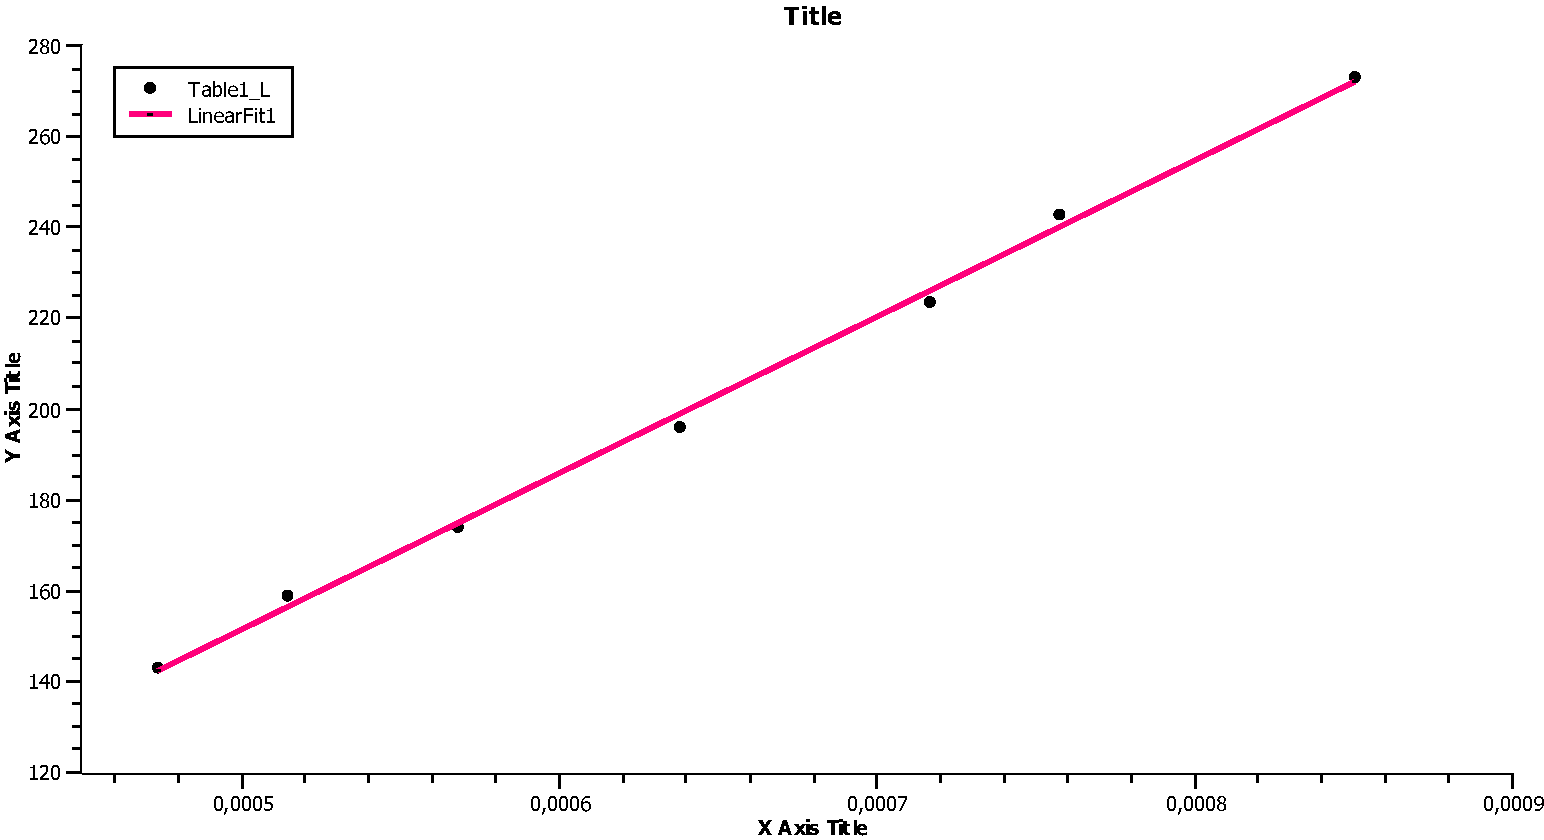
\includegraphics[width=.8\linewidth]{media/graphs/graph}
  \caption{Ajuste linear dos dados experimentais.}
  \label{fig:grafico}
\end{figure}

\textbf{Log de Extração de Dados - SciDAVis:}
\begin{verbatim}
Linear Regression fit of dataset: Table1_L, using function: A*x+B
From x = 0.000473484848484848 to x = 0.000850340136054422

B (y-intercept) = -20.4461 +/- 4.9031
A (slope) = 344089.7451 +/- 7454.3915
--------------------------------------------------------------------------------------
Chi^2 = 31.2156
R^2 = 0.9976
\end{verbatim}


\section{Discussão dos Resultados}

\subsection{Cálculo Experimental da Velocidade do Som}
A manipulação da variável independente para $x = \frac{1}{4f}$ transmuta a Equação 7 no formato linear $L = v_{\text{tubo}} \cdot \left(\frac{1}{4f}\right) - C$. Logo, o coeficiente angular da reta ($A$) fornece pontualmente a velocidade da onda. 

Efetuando a conversão das unidades de $\text{mm/s}$ para o SI ($\text{m/s}$):
$$v_{\text{tubo}} = A = 344089,74\text{ mm/s} \implies 344,09\text{ m/s}$$
$$\Delta v_{\text{tubo}} = \Delta A = 7454,39\text{ mm/s} \implies 7,45\text{ m/s}$$

A Velocidade Empírica Obtida resultou em $v_{\text{tubo}} = (344,1 \pm 7,5)\text{ m/s}$. O erro relativo perante a temperatura teórica ($345,88\text{ m/s}$) é de somente $0,52\%$. A excelente precisão estatística ($R^2 = 0,9976$) corrobora os dados da bancada e legitima o postulado do microclima de ar mais úmido dentro do tubo.

\subsection{Extração do Raio do Tubo (Correção de Helmholtz)}
A correção de Helmholtz para um tubo relaciona o intercepto da reta com o raio da seção transversal: $B \approx -0,6 R$. Utilizando o coeficiente linear extraído no SciDAVis ($B = -20,44\text{ mm}$), deduz-se o raio interno oculto do tubo d'água:
$$-20,44\text{ mm} = -0,6 \cdot R \implies R = \frac{20,44}{0,6} \approx 34,06\text{ mm} = 3,4\text{ cm}$$

A predição de um tubo com diâmetro interno de $\approx 6,8\text{ cm}$ é totalmente coerente com as provetas do experimento, validando as técnicas de regressão geométrica para medir propriedades fluidas.

\subsection{Restrições Sensoriais e Metodologia Ideal}
O experimento acarreta fontes inerentes de incerteza em sua execução prática:
\begin{enumerate}
    \item \textbf{Limitação da Percepção Humana:} A localização do ponto de máxima ressonância foi determinada exclusivamente pelo ouvido dos operadores. Como a audição humana é subjetiva e tem dificuldade em distinguir variações muito sutis de volume quando o som atinge seu pico, é fácil o experimentador se enganar ao cravar a medida, gerando uma incerteza natural de alguns milímetros na leitura da régua.
    \item \textbf{Menisco da Água:} A tensão superficial da água prejudica o alinhamento visual exato com a régua externa.
\end{enumerate}

Para obter resultados mais fidedignos e contornar essas limitações, sugere-se a adoção de um \textit{Tubo Seco com Êmbolo Móvel}. Substituindo a água por um pistão cilíndrico sólido horizontal, elimina-se o problema do curso mecânico da bancada. Além disso, a leitura da ressonância poderia ser automatizada por meio de um microfone acoplado a um software ou osciloscópio, eliminando completamente a subjetividade do ouvido humano na tomada de dados.

\section{Conclusão}
O experimento atingiu com maestria seus propósitos. O cálculo rigoroso pela equação dos gases ideais ditou uma referência teórica de $345,88\text{ m/s}$. Contornando as limitações físicas do tubo por meio da manipulação lógica de frequências, a regressão linear determinou a velocidade como $344,1\text{ m/s}$, evidenciando um pequeno desvio de $0,52\%$. 

A regressão linear não apenas forneceu a velocidade do som, mas também atestou a discrepância paramétrica das caixas de madeira ($2,40\text{ cm}$ de projeção do som) e isolou com precisão cirúrgica o raio da vidraria do experimento ($3,4\text{ cm}$). Os resultados atestam a extrema correlação analítica entre geometria de fluidos e instrumentação eletrônica na física acústica.


\bibliographystyle{plainnat}
\bibliography{refs}

\end{document}